\subsection{Independent Factorization on Phrasal-Anchoring}
\label{ssec:lex-phr:phr-factorization-analysis}
In the following, we focus on the first two main challenge in
independent factorization: \textbf{output decomposition} and
\textbf{input decomposition} on phrasal-anchoring. We leave the
\textbf{factor modelling} into the next part. We consider the same
sentence example~\dquoted{Pierre Vinken, 61 years old, will join the board as
  a nonexecutive director Nov.29.} and its corresponding UCCA graph as
shown in~\autoref{fig:bg:ucca}. We introduce the details of
independent factorization for UCCA and other pharsal-anchoring
representations.

\subsubsection{Output Decomposition}
\label{sssec:lex-phr:phr-output-decomposition}
\begin{figure}[!tbp]
  \centering
  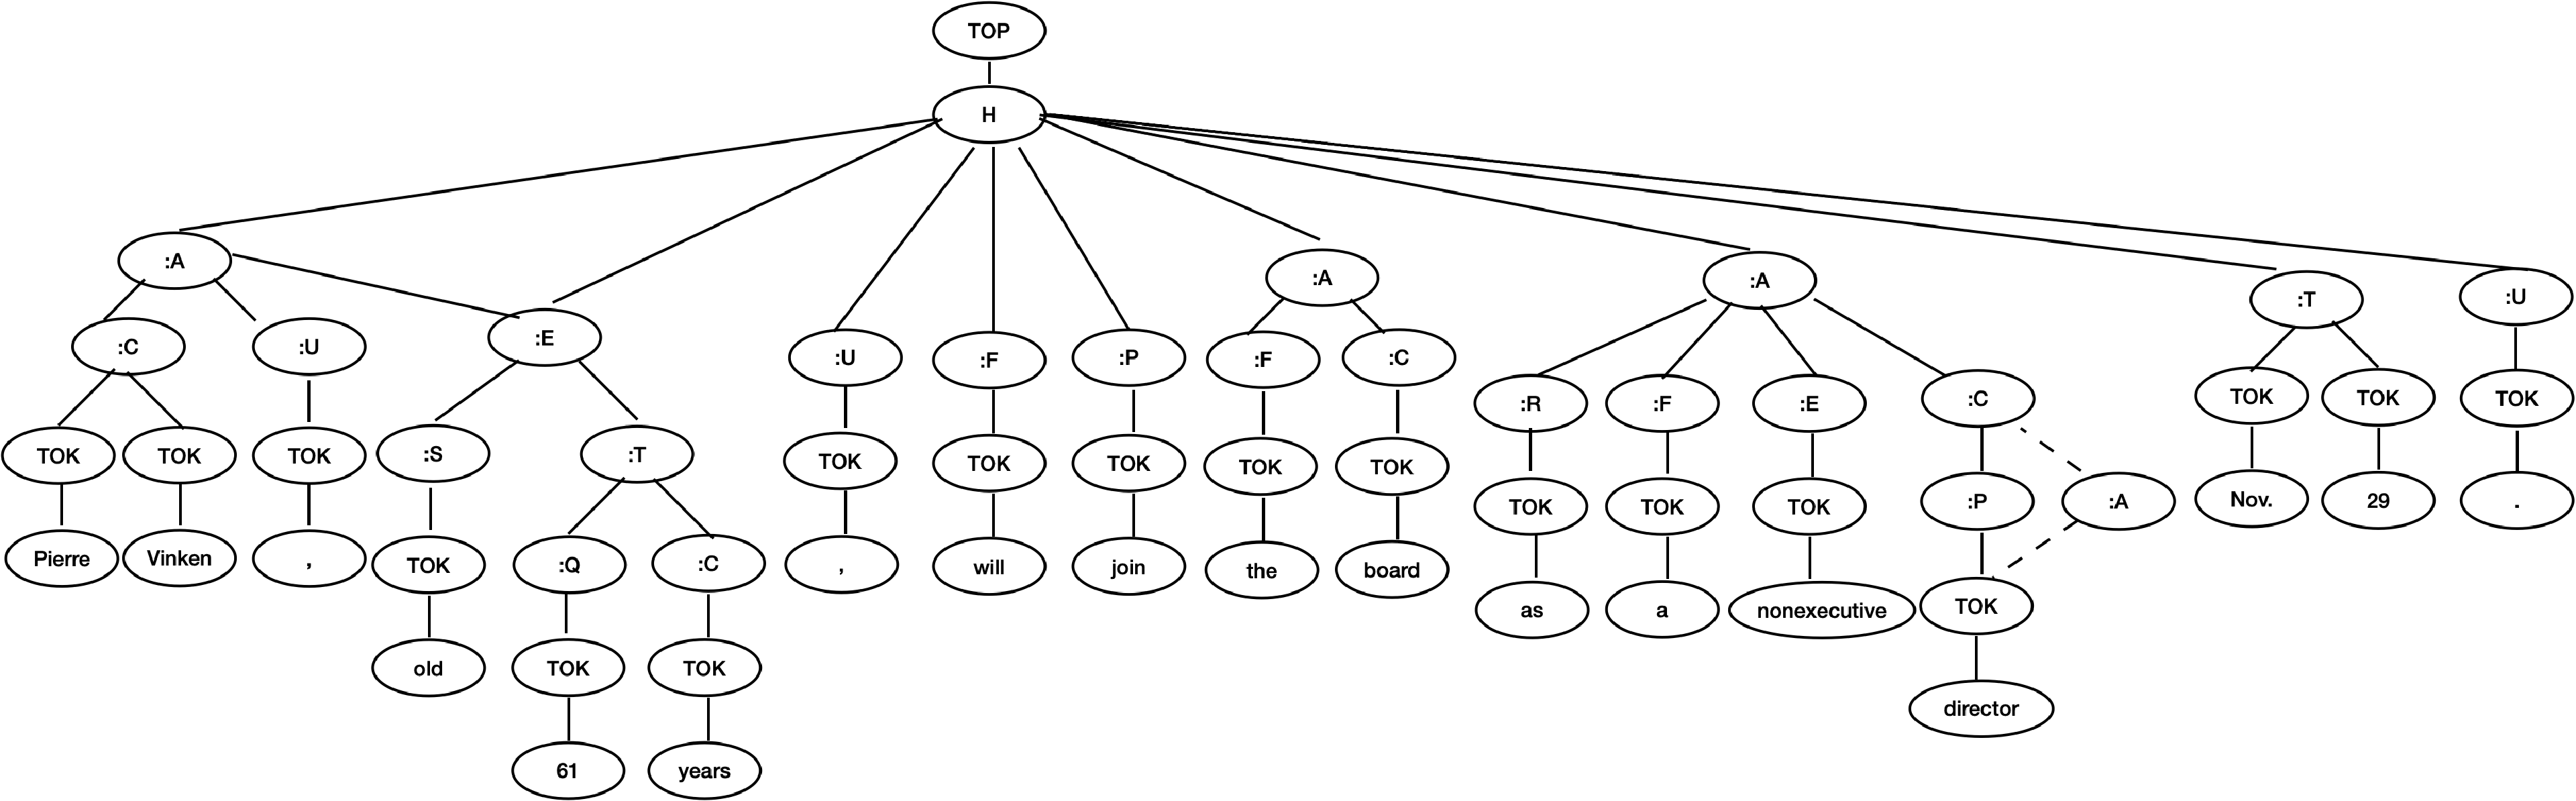
\includegraphics[width=0.98\textwidth]{pierre-ucca-decomposition.pdf}
  \caption{\label{fig:lex-phr:ucca-decomposition} UCCA decomposition
    for the sentence \#20001001.}
\end{figure}

After the above transformation, as shown in the
\autoref{fig:lex-phr:ucca-decomposition} the labelled nodes in UCCA
are linked into a hierarchical structure, with edges going between
parent and child nodes. With certain exceptions~(\eg, remote edges,
the dashed line to the node \tquoted{:A} with a second parent of node
\tquoted{director}), the majority of the UCCA graphs are tree-like
structures. In this disseration, because the remote edge are rare, we
ignore all the exception to simplfy the modeling. According to the
position as well as the anchoring style, nodes in UCCA can naturally
classified into the following two types:

\begin{inparaenum}
\item \textbf{Terminal nodes} are the leaf semantic
  concepts anchored to individual lexical units in the sentence

\item \textbf{Nonterminal nodes} are usually anchored to a span with
  more than one lexical units, thus usually overlapped with the
  anchoring of terminal nodes.
\end{inparaenum}

Hence, it is natural that we can decompose the transformed UCCA tree
into two set of nodes, both of them can be produced from the
corresponding lexical units or phrases. However, more challenges
exists on how to generate the input segments that can produce those
output decompostions.

\subsubsection{Input Decomposition and Alignments Discovery}
\label{sssec:lex-phr:phr-input-decomposition}
Different from the lexical anchoring without overlapping, UCCA may
align to larger overlapped word spans which involves syntactic or
semantic pharsal structure. Further mode, the phrasal decomposition
and the alignment model is provided in training data. However, we have
no idea on how to factorize the input during inference.

In lexical anchoring, the input decomposition are handled with a
rule-based preprocessing step. However, there is no clear rules how to
decompose a sentence into a structure similar with consistuent tree
structure. Luckily, we have many previous studies on how to parse a
sentence into a constituent tree, which inspired us that we can model
the input decomposition jointly with the factor modelling part. We
leave more details of the model for joint input decomposition and
factor modeling in~\autoref{ssec:phr:cky}.

%%% Local Variables:
%%% mode: latex
%%% TeX-master: "../../dissertation-main.ltx"
%%% End:
